% Plantilla de Memoria
% Modificación de una plantilla de Latex de Nicolas Diaz para adaptarla 
% al castellano y a las necesidades de escribir informática y matemáticas.
%
% Editada por: Mario Román
%
% License:
% CC BY-NC-SA 3.0 (http://creativecommons.org/licenses/by-nc-sa/3.0/)
%%%

%%%%%%%%%%%%%%%%%%%%%%%%%%%%%%%%%%%%%%%%%
% Thin Sectioned Essay
% LaTeX Template
% Version 1.0 (3/8/13)
%
% This template has been downloaded from:
% http://www.LaTeXTemplates.com
%
% Original Author:
% Nicolas Diaz (nsdiaz@uc.cl) with extensive modifications by:
% Vel (vel@latextemplates.com)
%
% License:
% CC BY-NC-SA 3.0 (http://creativecommons.org/licenses/by-nc-sa/3.0/)
%
%%%%%%%%%%%%%%%%%%%%%%%%%%%%%%%%%%%%%%%%%

%----------------------------------------------------------------------------------------
%	PAQUETES Y CONFIGURACIÓN DEL DOCUMENTO
%----------------------------------------------------------------------------------------

%%% Configuración del papel.
% microtype: Tipografía.
% mathpazo: Usa la fuente Palatino.
\documentclass[a4paper, 11pt]{article}
\usepackage[protrusion=true,expansion=true]{microtype}
\usepackage{mathpazo}

% Indentación de párrafos para Palatino
\setlength{\parindent}{0pt}
  \parskip=8pt
\linespread{1.05} % Change line spacing here, Palatino benefits from a slight increase by default


%%% Castellano.
% noquoting: Permite uso de comillas no españolas.
% lcroman: Permite la enumeración con numerales romanos en minúscula.
% fontenc: Usa la fuente completa para que pueda copiarse correctamente del pdf.
\usepackage[spanish,es-noquoting,es-lcroman]{babel}
\usepackage[utf8]{inputenc}
\usepackage[T1]{fontenc}
\selectlanguage{spanish}
\usepackage[scr=rsfs]{mathalpha}
\newcommand\userinput[1]{\textbf{#1}}


%%% Gráficos
\usepackage{graphicx} % Required for including pictures
\usepackage{wrapfig} % Allows in-line images
\usepackage[usenames,dvipsnames]{color} % Coloring code


%%% Matemáticas
\usepackage{amsmath}
\usepackage{alltt}


%%% Código fuente
\usepackage{listings}
\usepackage{fancyvrb}
\usepackage{ dsfont }

%%% Tablas en su sitio
\usepackage{float}
\usepackage{ amssymb }
\usepackage{booktabs}

%%% Bibliografía
\makeatletter
\renewcommand\@biblabel[1]{\textbf{#1.}} % Change the square brackets for each bibliography item from '[1]' to '1.'
\renewcommand{\@listI}{\itemsep=0pt} % Reduce the space between items in the itemize and enumerate environments and the bibliography


%----------------------------------------------------------------------------------------
%	TÍTULO
%----------------------------------------------------------------------------------------
% Configuraciones para el título.
% El título no debe editarse aquí.
\renewcommand{\maketitle}{
  \begin{flushright} % Right align
  
  {\LARGE\@title} % Increase the font size of the title
  \\ \@date % Date
  \vspace{50pt} % Some vertical space between the title and author name
  
  
  {\large\@author} % Author name
  \\
  \vspace{40pt} % Some vertical space between the author block and abstract
  \end{flushright}
}

%% Título
\title{\textbf{Informe Final EMV}}  % Subtitle

\date{Curso 2023/2024} % Date

\author{
	Doble Grado en Ingeniería Informática y Matemáticas
}





%----------------------------------------------------------------------------------------
%	DOCUMENTO
%----------------------------------------------------------------------------------------

\begin{document}

\maketitle % Print the title section
\pagebreak

%% Resumen (Descomentar para usarlo)
\renewcommand{\abstractname}{Resumen} % Uncomment to change the name of the abstract to something else
%\begin{abstract}
% Resumen aquí
%\end{abstract}

%% Palabras clave
%\hspace*{3,6mm}\textit{Keywords:} lorem , ipsum , dolor , sit amet , lectus % Keywords
%\vspace{30pt} % Some vertical space between the abstract and first section


%% Índice
{\parskip=2pt
  \tableofcontents
}
\pagebreak

%%% Inicio del documento

\section{Introducción}

El \textbf{objetivo principal} de este estudio es utilizar técnicas de \textbf{aprendizaje automático} para desarrollar un modelo predictivo \textbf{preciso}. Este modelo buscará establecer una relación entre las diferentes variables sociodemográficas y escolares proporcionadas en el dataset (como sexo, edad, tiempo de estudio, apoyo educativo recibido, entre otros) y la nota final obtenida por los estudiantes en Matemáticas.

El uso de técnicas de \textbf{aprendizaje automático}, como modelos de clasificación, permitirá construir un modelo robusto que pueda predecir con \textbf{precisión} las calificaciones de los estudiantes en función de las variables proporcionadas en el dataset. Esto puede ser de gran utilidad para profesores, administradores escolares y responsables de políticas educativas para mejorar el rendimiento estudiantil y brindar un apoyo más personalizado a los alumnos en sus estudios de Matemáticas.

El propósito de este análisis es \textbf{identificar las variables predictoras más relevantes} y determinar cómo influyen en el rendimiento académico en Matemáticas, así como hacer una \textbf{reducción de la dimensión}. Al comprender mejor estas relaciones, se busca no solo predecir las calificaciones futuras de los estudiantes, sino también obtener información útil para tomar decisiones educativas, identificar áreas de mejora y diseñar estrategias de apoyo más efectivas para los estudiantes.

\section{Materiales y métodos}

\subsection{Materiales}

Para realizar este estudio se ha tomado una base de datos. Esta contiene información sobre 31 indicadores medidos en 395 estudiantes. Estos indicadores son los siguientes:

\begin{itemize}
\item \textbf{school}: Centro escolar del estudiante
\item \textbf{sex}: Sexo del estudiante
\item \textbf{age}: Edad del estudiante
\item \textbf{address}: Tipo de dirección de vivienda del estudiante
\item \textbf{famsize}: Número de miembros de la familia del estudiante
\item \textbf{Pstatus}: Estado de convivencia de los padres del estudiante
\item \textbf{Medu}: Educación de la madre del estudiante
\item \textbf{Fedu}: Educación del padre del estudiante
\item \textbf{Mjob}: Trabajo de la madre del estudiante
\item \textbf{Fjob}: Trabajo del padre del estudiante
\item \textbf{reason}: Motivo del estudiante por el cual eligió su centro escolar
\item \textbf{guardian}: Tutor del estudiante
\item \textbf{traveltime}: Tiempo de viaje de casa del estudiante al centro escolar
\item \textbf{studytime}: Tiempo de estudio semanal del estudiante
\item \textbf{failures}: Número de materias suspendidas en el pasado
\item \textbf{schoolsup}: El estudiante recibe apoyo educativo adicional
\item \textbf{famsup}: El estudiante recibe apoyo educativo familiar
\item \textbf{paid}: El estudiante recibe clases extras pagadas de la asignatura Matemáticas
\item \textbf{activities}: El estudiante está apuntado en actividades extracurriculares
\item \textbf{nursery}: El estudiante asistió de pequeño a la guardería
\item \textbf{higher}: El estudiante quiere cursar estudios superiores
\item \textbf{internet}: El estudiante tiene acceso a Internet en casa
\item \textbf{romantic}: El estudiante se encuentra en una relación de pareja
\item \textbf{famrel}: Calidad de las relaciones familiares del estudiante
\item \textbf{freetime}: Cantidad de tiempo libre que posee el estudiante después del colegio
\item \textbf{goout}: Frecuencia con la que el estudiante sale a la calle con sus amigos
\item \textbf{Dalc}: Cantidad de consumo de alcohol del estudiante en jornada laboral
\item \textbf{Walc}: Cantidad de consumo de alcohol del estudiante en el fin de semana
\item \textbf{health}: Estado de salud actual del estudiante
\item \textbf{absences}: Número de veces que el estudiante ha faltado al colegio
\item \textbf{G3}: Nota final del estudiante en la asignatura Matemáticas
\end{itemize}

\textbf{Se ha codificado el dataset}, de forma que \textbf{todas las variables sean de tipo numérico} para poder trabajar con ellas más fácilmente.

Además, se muestran tablas donde aparece una visión general de los estadísticos de cada variable:

\begin{center}
\begin{tabular}{lcccccc}
\toprule
& Mínimo & Primer Cuartil & Mediana & Tercer Cuartil & Máximo & Rango \\ 
\midrule
school       & 0.0000 & 0.0000 & 0.0000 & 0.0000 & 1.0000 & 1.0000 \\ 
sex          & 0.0000 & 0.0000 & 0.0000 & 1.0000 & 1.0000 & 1.0000 \\ 
age          & 15.0   & 16.0   & 17.0   & 18.0   & 22.0   & 7.0000 \\ 
address      & 0.0000 & 0.0000 & 0.0000 & 0.0000 & 1.0000 & 1.0000 \\ 
famsize      & 0.0000 & 0.0000 & 1.0000 & 1.0000 & 1.0000 & 1.0000 \\ 
Pstatus      & 0.0000 & 0.0000 & 0.0000 & 0.0000 & 1.0000 & 1.0000 \\ 
Mjob         & 0.0000 & 2.0000 & 2.499  & 4.0000 & 4.0000 & 4.0000 \\ 
reason       & 0.0000 & 0.0000 & 1.0000 & 2.0000 & 3.0000 & 3.0000 \\ 
traveltime   & 1.0000 & 1.0000 & 1.0000 & 2.0000 & 4.0000 & 3.0000 \\ 
studytime    & 1.0000 & 2.0000 & 2.0000 & 2.0230 & 4.0000 & 3.0000 \\ 
failures     & 0.0000 & 0.0000 & 0.0000 & 0.0000 & 3.0000 & 3.0000 \\ 
schoolsup    & 0.0000 & 1.0000 & 1.0000 & 1.0000 & 1.0000 & 1.0000 \\ 
famsup       & 0.0000 & 0.0000 & 0.0000 & 1.0000 & 1.0000 & 1.0000 \\ 
paid         & 0.0000 & 0.0000 & 1.0000 & 1.0000 & 1.0000 & 1.0000 \\ 
activities   & 0.0000 & 0.0000 & 0.0000 & 1.0000 & 1.0000 & 1.0000 \\ 
nursery      & 0.0000 & 0.0000 & 0.0000 & 0.0000 & 1.0000 & 1.0000 \\ 
higher       & 0.0000 & 0.0000 & 0.0000 & 0.0000 & 1.0000 & 1.0000 \\ 
internet     & 0.0000 & 0.0000 & 0.0000 & 0.0000 & 1.0000 & 1.0000 \\ 
romantic     & 0.0000 & 0.0000 & 1.0000 & 1.0000 & 1.0000 & 1.0000 \\ 
famrel       & 1.0000 & 4.0000 & 4.0000 & 5.0000 & 5.0000 & 4.0000 \\ 
freetime     & 1.0000 & 3.0000 & 3.0000 & 4.0000 & 5.0000 & 4.0000 \\ 
goout        & 1.0000 & 2.0000 & 3.0000 & 4.0000 & 5.0000 & 4.0000 \\ 
Dalc         & 1.0000 & 1.0000 & 1.0000 & 2.0000 & 5.0000 & 4.0000 \\ 
Walc         & 1.0000 & 1.0000 & 2.0000 & 3.0000 & 5.0000 & 4.0000 \\ 
health       & 1.0000 & 3.0000 & 4.0000 & 5.0000 & 5.0000 & 4.0000 \\ 
absences     & 0.0000 & 0.0000 & 4.0000 & 8.0000 & 75.000 & 75.0000 \\ 
G3           & 0.0000 & 8.0000 & 11.0   & 14.0   & 20.0   & 20.0000 \\ 
\bottomrule
\end{tabular}
\textbf{Tabla 1} Estadísticas de posición de las variables


\centering
\begin{tabular}{lcccccc}
\toprule
& Media & Varianza & Desv. típica & Co. variación & Co. asimetría & Co. curtosis \\ 
\midrule
school       & 0.1165 & 0.1031 & 0.3212 & 2.7579 & 2.3823 & 3.6848 \\ 
sex          & 0.4734 & 0.2499 & 0.4999 & 1.0559 & 0.1061 & -1.9938 \\ 
age          & 16.7   & 1.6283 & 1.2760 & 0.0764 & 0.4627 & -0.0314 \\ 
address      & 0.2228 & 0.1736 & 0.4166 & 1.8702 & 1.3273 & -0.2388 \\ 
famsize      & 0.7114 & 0.2058 & 0.4537 & 0.6377 & -0.9295 & -1.1389 \\ 
Pstatus      & 0.1038 & 0.0933 & 0.3054 & 2.9421 & 2.5882 & 4.7108 \\ 
Mjob         & 2.499  & 1.9499 & 1.3964 & 0.5588 & -0.4715 & -0.9881 \\ 
reason       & 1.273  & 0.9352 & 0.9671 & 0.7594 & 0.0383 & -1.1256 \\ 
traveltime   & 1.448  & 0.4865 & 0.6975 & 0.4817 & 1.5948 & 2.2727 \\ 
studytime    & 2.023  & 0.6086 & 0.7802 & 0.3856 & 0.6884 & 0.4379 \\ 
failures     & 0.3342 & 0.553  & 0.7437 & 2.2253 & 2.3689 & 4.8864 \\ 
schoolsup    & 0.8709 & 0.1127 & 0.3358 & 0.3855 & -2.2037 & 2.8636 \\ 
famsup       & 0.3873 & 0.2379 & 0.4878 & 1.2592 & 0.4608 & -1.7922 \\ 
paid         & 0.5418 & 0.2489 & 0.4989 & 0.9208 & -0.1670 & -1.9771 \\ 
activities   & 0.4911 & 0.2506 & 0.5006 & 1.0192 & 0.0353 & -2.0038 \\ 
nursery      & 0.2051 & 0.1634 & 0.4043 & 1.9714 & 1.4555 & 0.1187 \\ 
higher       & 0.05063 & 0.0482 & 0.2195 & 4.3356 & 4.0836 & 14.7133 \\ 
internet     & 0.1671 & 0.1395 & 0.3735 & 2.2355 & 1.7780 & 1.1643 \\ 
romantic     & 0.6658 & 0.2231 & 0.4723 & 0.7093 & -0.7004 & -1.5132 \\ 
famrel       & 3.944  & 0.8034 & 0.8967 & 0.2273 & -0.9447 & 1.0895 \\ 
freetime     & 3.235  & 0.9977 & 0.9999 & 0.3087 & -0.1621 & -0.3267 \\ 
goout        & 3.109  & 1.2393 & 1.1133 & 0.3581 & 0.1156 & -0.7869 \\ 
Dalc         & 1.481  & 0.7934 & 0.8907 & 0.6014 & 2.1742 & 4.6454 \\ 
Walc         & 2.291  & 1.6587 & 1.2879 & 0.5621 & 0.6073 & -0.8072 \\ 
health       & 3.554  & 1.9329 & 1.3903 & 0.3911 & -0.4909 & -1.0265 \\ 
absences     & 5.709  & 64.0495 & 8.0031 & 1.4019 & 3.6437 & 21.3065 \\ 
G3           & 10.42  & 20.9896 & 4.5814 & 0.4399 & -0.7271 & 0.3661 \\ 
\bottomrule
\end{tabular}

\textbf{Tabla 2} Estadísticas de dispersión de las variables

\end{center}

\subsection{Métodos Estadísticos}

Primero, se ha realizado un \textbf{análisis exploratorio} previo de los datos para detectar \textbf{valores pérdidos} y \textbf{valores atípicos (outliers)}. Se han tomado distintas decisiones para abordar estos valores anómalos.

\newpage

\begin{itemize}
\item Para variables con \textbf{más de un 5\%} de valores pérdidos se ha analizado el patrón aleatorio de los mismos estudiando la \textbf{homogeneidad} según grupos con otras variables sin datos perdidos. Como las variables eran cuantitativas, se ha utilizado un \textbf{test de Student}.

\item En el caso de las variables con \textbf{outliers}, se han detectado utilizando gráficos \textit{boxplot} y se ha decidido sustituirlos por la \textbf{media} (al ser variables cuantitativas).
\end{itemize} 

Después, se ha realizado un análisis \textbf{descriptivo numérico clásico} presentando medidas estadísticas de posición, dispersión y forma. Estas medidas han proporcionado una visión más detallada de la distribución de los datos, permitiendo una \textbf{comprensión} más profunda de su estructura y comportamiento.

En tercer lugar, se han aplicado diversas técnicas de análisis multivariante comprobando los supuestos para cada una de ellas:

\begin{itemize}
\item \textbf{Comprobación de la correlación entre datos}: Se ha realizado una \textbf{evaluación exhaustiva} de la correlación entre los datos, tanto a nivel poblacional como a nivel muestral. Para confirmar si las correlaciones eran significativamente distintas de cero a nivel poblacional se ha aplicado el \textbf{contraste de esfericidad de Bartlett}. A nivel muestral, se ha examinado la estructutra de las correlaciones utilizando la \textbf{matriz de correlaciones y la matriz policrítica}, así como otras representaciones gráficas. Estas representaciones nos han proporcionado una visión detallada de las relaciones entre las variables.

\item \textbf{Comprobación de la normalidad univariante}: Se ha realizado una exploración gráfica mediante \textbf{histogramas y gráficos qqplots}. Estos gráficos nos han proporcionado una perspectiva inicial sobre si las variables unidimensionales seguían una distribución normal. No obstante, la conclusión final sobre la normalidad se obtuvo utilizando el test de \textbf{Shapiro-Willks}.


\item \textbf{Comprobación de la normalidad multivariante}: Se han utilizado test de hipotésis como el de \textbf{Royston} y el de \textbf{Henze-Zirkler}.
\end{itemize}

\newpage

\section{Resultados}

\textbf{Primero}, hemos tenido cuidado con las variables codificadas que eran \textbf{categóricas} originalmente y que tienen más de dos niveles de respuesta porque quizá no interese incluirlas. En nuestro caso, estas son \textbf{Medu}, \textbf{Fedu}, \textbf{Mjob}, \textbf{Fjob}, \textbf{reason} y \textbf{guardian}. Para decidir si las incluímos o no, deberíamos preguntar al diseñador del dataset si esas variables son \textbf{relevantes} para el problema bajo estudio. Como no podemos contactar con él, asumimos que lo son. Así, una forma de ver si pueden ser útiles es hacer un \textbf{análisis descriptivo} de ellas y ver si los niveles están compensados (más o menos hay el mismo número de individuos en cada uno). Si lo están es una variable que podría aportar \textbf{información}, pero si hay algún nivel muy bajo o si todo se acumula en un nivel, habría que plantearse descartar la variable. Tras hacer este análisis hemos decidido eliminar las variables: \textbf{Medu}, \textbf{Fedu}, \textbf{Fjob} y \textbf{guardian}.

Luego, se estudian los \textbf{valores perdidos} en el dataset. Se observa que la variable \textbf{Mjob} tiene menos de un 5 \%, por lo que estos se pueden sustituir directamente por la \textbf{media} de los valores conocidos. Sin embargo, la variable continua \textbf{studytime} tiene más de un 5 \% de valores perdidos, así que se debe estudiar la \textbf{aleatoriedad} de los mismos mediante un test de Student, dando como resultado que \textbf{no se puede rechazar la hipótesis nula} de homogeneidad. En consecuencia, se concluye que el patrón es \textbf{aleatorio}. Por tanto, se ha decidido \textbf{sustituir} los valores perdidos de esta variable por la media de los valores conocidos.

También se detecta la presencia de \textbf{outliers}, y se toma la decisión de \textbf{sustituirlos por la media} de sus variables.

Tras el tratamiento de \textbf{outliers}, hay algunas variables que tienen el mismo valor para todos los registros, haciendo que su \textbf{varianza} sea cero, lo cual nos da problemas, por ejemplo, el test de \textbf{normalidad} univariante de Shapiro-Willks. En concreto, estas variables son \textbf{school}, \textbf{address}, \textbf{Pstatus}, \textbf{failures}, \textbf{schoolsup}, \textbf{nursery}, \textbf{higher} e \textbf{internet}. Por ello, como tenemos un gran número de variables, se ha decidido \textbf{eliminarlas}. Como resultado, trabajamos en lo que sigue con 19 variables (recordemos que inicialmente había 31 variables).

Pasamos a estudiar la \textbf{independencia} entre variables con el test de Bartlett, dando como resultado que no se puede rechazar la hipótesis de independencia entre variables. Por tanto, no tiene sentido plantearse una \textbf{reducción de la dimensión} del conjunto de variables mediante un \textbf{Análisis de Componentes Principales} o un \textbf{Análisis Factorial}.


Además, se ha concluido mediante el test de Saphiro-Willks que no se puede afirmar que haya \textbf{normalidad univariante} para la mayoría de las variables condicionadas a cada modalidad de la variable cualitativa estudiada en el Análisis Discriminante.

Se han usado también distintos tests para comprobar la \textbf{normalidad multivariante}, dando como resultado que tampoco se puede afirmar que la haya. Debido a la ausencia de estas hipótesis de normalidad, se ha decidido no tener en cuenta los resultados del Análisis Discriminante Lineal, pero sí los del Análisis Discriminante Cuadrático, por ser \textbf{más robusto} a esta ausencia.

Para el Análisis Discriminante se ha definido una variable respuesta categórica a partir de la \textbf{calificación del estudiante} almacenada en la variable G3. Esta variable categórica toma el valor aprobado si el valor de G3 es mayor o igual a 10.0 y suspenso si es menor a 10.0. Por los motivos expuestos en el párrafo anterior, vamos a centrarnos exclusivamente en los resultados del Análisis Discriminante Cuadrático, para el cual se ha obtenido un porcentaje de error del 31.65 \% (es decir, tenemos un porcentaje de acierto del 68.35 \%).

A continuación, se muestran los tres modelos de clasificación cuadráticos con dos predictores que tienen un porcentaje de error más bajo:

\begin{figure}[h]
\centering
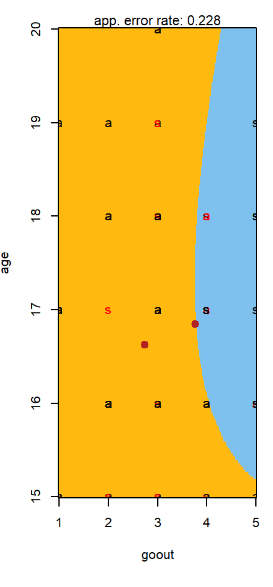
\includegraphics[height=7cm]{capturaemv1.png}
\hfill
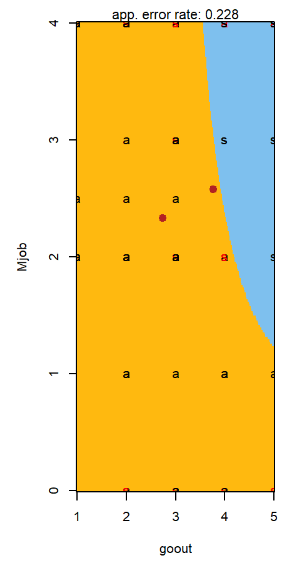
\includegraphics[height=7cm]{capturaemv2.png}
\hfill
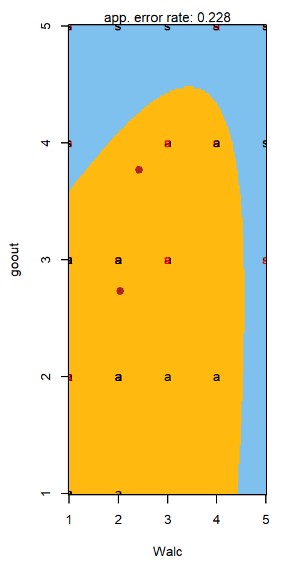
\includegraphics[height=7cm]{capturaemv3.png}
\caption{Modelos de clasificación cuadráticos con dos predictores que tienen un porcentaje de error más bajo}
\label{fig:tres_imagenes}
\end{figure}

\newpage

Observamos que estos tres modelos con dos predictores tiene un porcentaje de error \textbf{más bajo que el modelo en el que usamos todas las variables} del dataset como predictores (excluyendo obviamente la variable G3, usada para definir la variable respuesta). Por tanto, nos interesará utilizar \textbf{menos predictores} con el fin de conseguir el menor porcentaje de error posible, además de un \textbf{menor coste} en recogida y computación de los datos.

\section{Discusión}

El estudio se enfocó en datos correspondientes a 31 variables, los cuales fueron evaluados en 395 estudiantes diferentes. El propósito principal de la investigación consistió en \textbf{implementar una reducción de la dimensionalidad y determinar las variables predictoras más relevantes} para determinar si un estudiante aprueba o suspende.

Tras aplicar el test correspondiente, no pudimos descartar la independencia de las variables. Por tanto, \textbf{no realizamos una reducción de la dimensión} mediante el procedimiento de Análisis de Componentes Principales o Análisis Factorial.

Finalmente se ha querido \textbf{clasificar} los datos en función de la calificación final del estudiante en la asignatura de Matemáticas, teniendo en cuenta el resto de variables del dataset como variables predictoras y con el objetivo de, dados los datos de un nuevo estudiante, poder determinar si aprueba o suspende. Entonces, mediante un Análisis Discriminante Cuadrático se ha obtenido un \textbf{método de clasificación} para nuevas observaciones.

Cabe destacar que, en base a los resultados obtenidos, la \textbf{variable goout} (frecuencia con la que el estudiante sale a la calle con sus amigos) es muy \textbf{influyente} a la hora de determinar la calificación final del estudiante.

\newpage

\section{Conclusión}

En este trabajo se ha estudiado una serie de datos relacionados con el ámbito social y escolar de diferentes estudiantes. Se ha obtenido un \textbf{método de clasificación} de la calificación final del estudiante en la asignatura de Matemáticas en función de dichos datos, lo cual puede ayudar a mejorar las políticas educativas de los centros escolares con el fin de \textbf{incrementar el rendimiento académico} y brindar un apoyo más personalizado a los alumnos en sus estudios de Matemáticas en función de la \textbf{situación} de cada estudiante.

Como limitaciones existentes, muchos supuestos necesarios para aplicar algunas técnicas \textbf{no se dan}, y aunque se ha podido decir poco, \textbf{no se pueden desprender más conclusiones} de los datos mediante las técnicas propuestas. Sin embargo, se considera que usando otras técnicas más robustas como \textbf{regresión logística} se podrían obtener mejores resultados.


\end{document}